\section{Methodology}
\begin{frame}
    \sectionpage
\end{frame}

\begin{frame}
    \frametitle{Lasso}

    how to do?

    what's the results?

    weakness? drawbacks?
\end{frame}

\begin{frame}
    \frametitle{Result of LASSO}

    \begin{figure}[h]
        \centering
        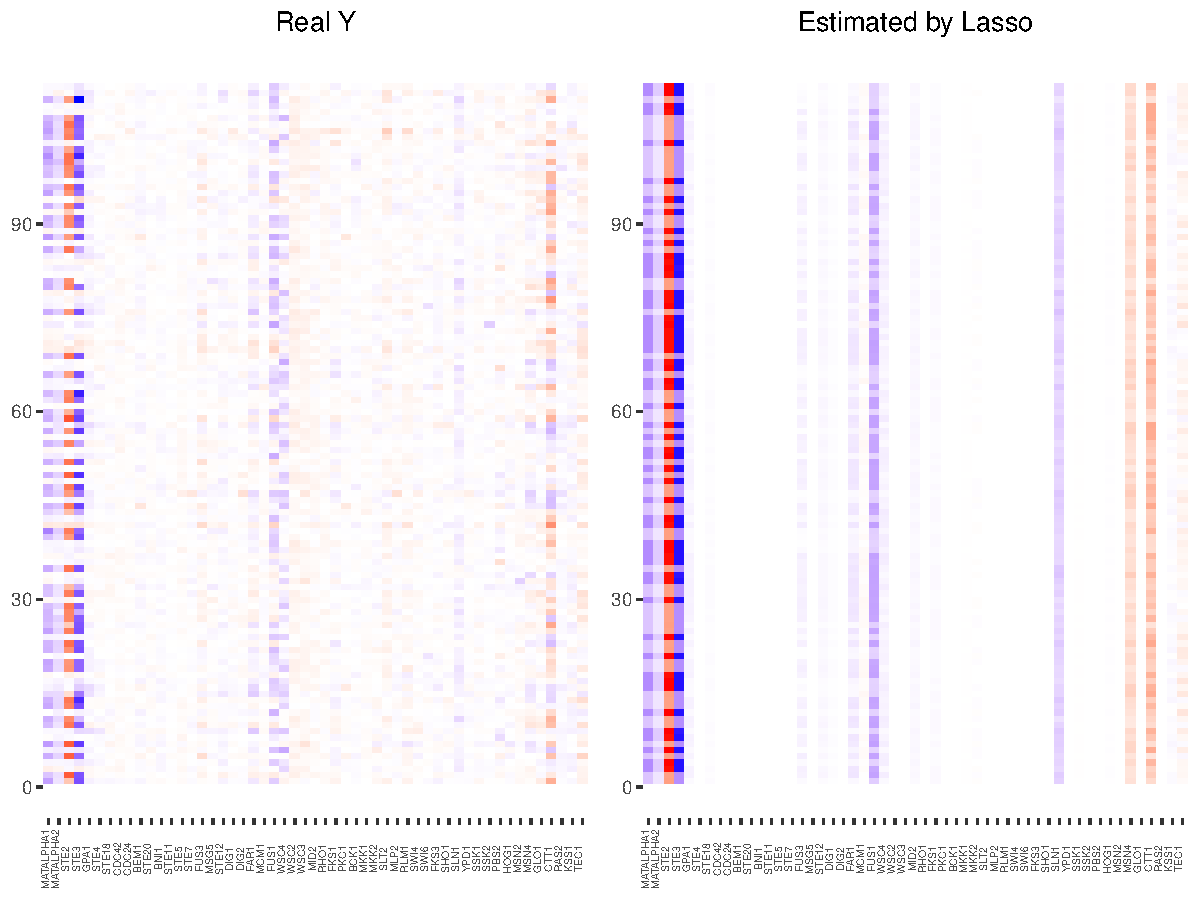
\includegraphics[width=0.8\textwidth]{./figs/lasso.pdf}
        \caption{Heatmaps of real $Y$ and $\hat{Y}$ by LASSO}
    \end{figure}    

\end{frame}

\begin{frame}{Multi-response regression}
    how to do? 

    what's the result?

    goodness? advantages?
    
\end{frame}

\begin{frame}
    \frametitle{Result of SOFAR}
    \begin{figure}[h]
        \centering
        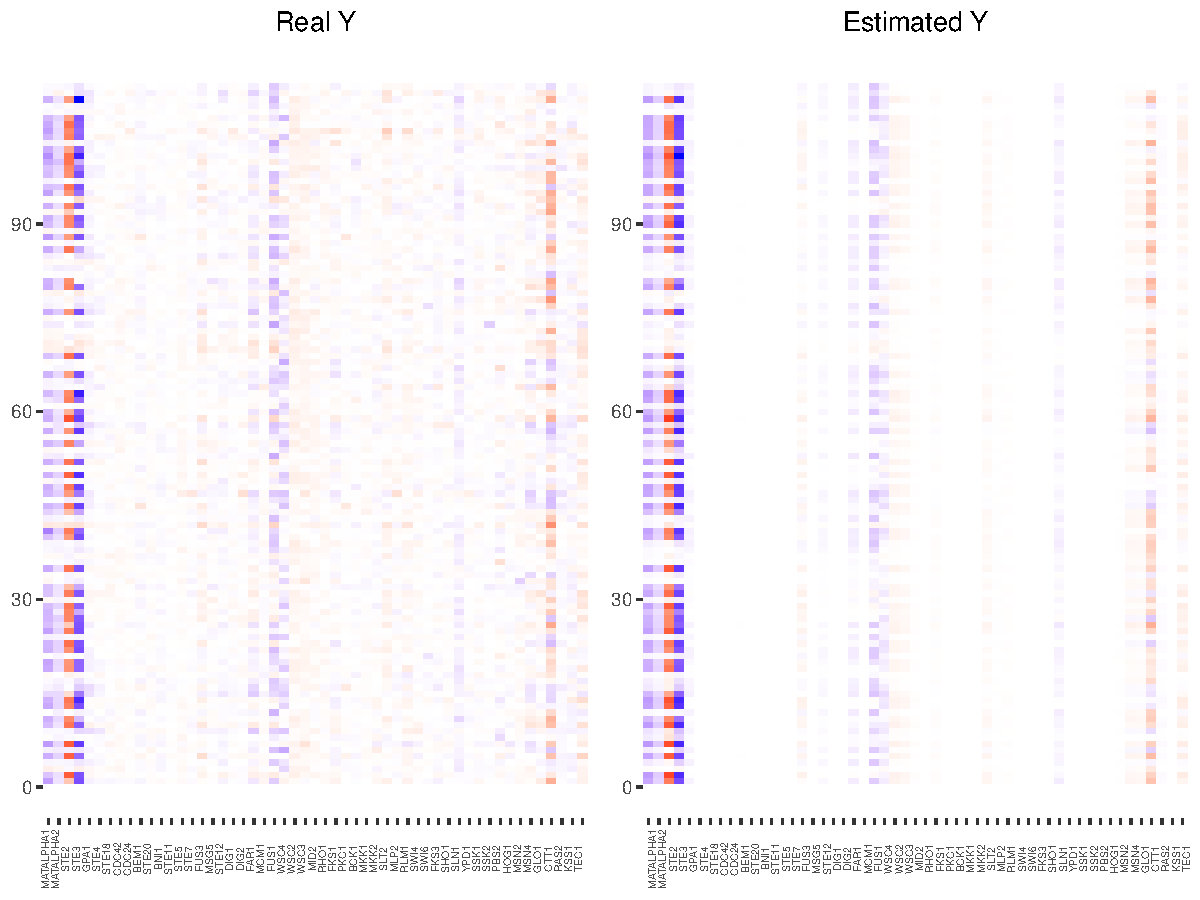
\includegraphics[width=0.8\textwidth]{./figs/heatmap1.pdf}
        \caption{Heatmaps of real $Y$ and $\hat{Y}$ by SOFAR}
    \end{figure}
\end{frame}

\begin{frame}
    \frametitle{Result of SOFAR}
    \begin{figure}[h]
        \centering
        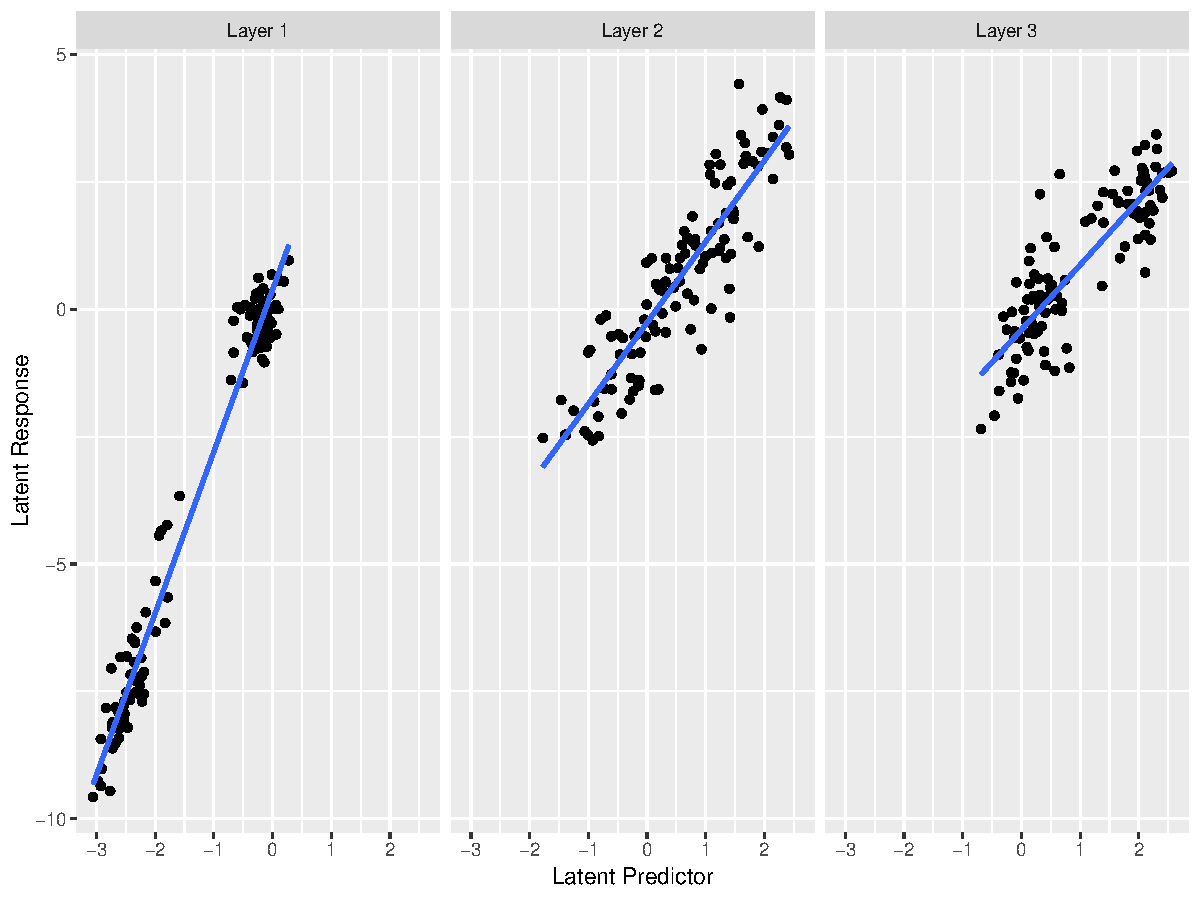
\includegraphics[width=0.75\textwidth]{./figs/latent1.pdf}
        \caption{Scatterplots of the latent responses versus the latent predictors in three SVD layers for the yeast data estimated by the SOFAR method}
    \end{figure}
\end{frame}


\begin{frame}
    \frametitle{Further Reduce Dimension of Markers}

    We performed a marginal gene-marker association analysis to identify markers that are associated with the expression levels of at least two genes with a p-value less than $0.05$, resulting in a total of $p = 776$ markers.

    Remove 

\end{frame}


\begin{frame}
    \frametitle{Result of SOFAR after Reduction}
    \begin{figure}[h]
        \centering
        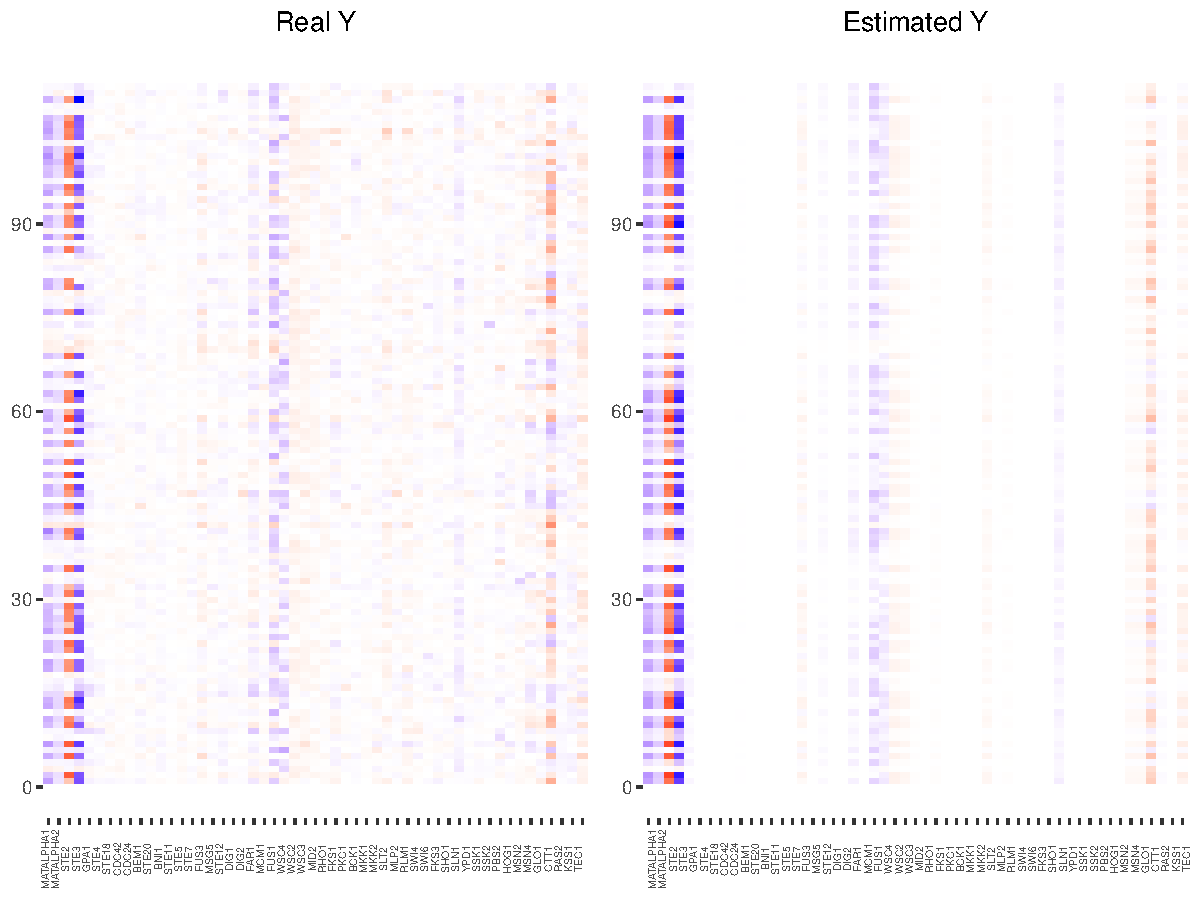
\includegraphics[width=0.8\textwidth]{./figs/heatmap2.pdf}
        \caption{Heatmaps of real $Y$ and $\hat{Y}$ by SOFAR}
    \end{figure}
\end{frame}

\begin{frame}
    \frametitle{Result of SOFAR after Reduction}
    \begin{figure}[h]
        \centering
        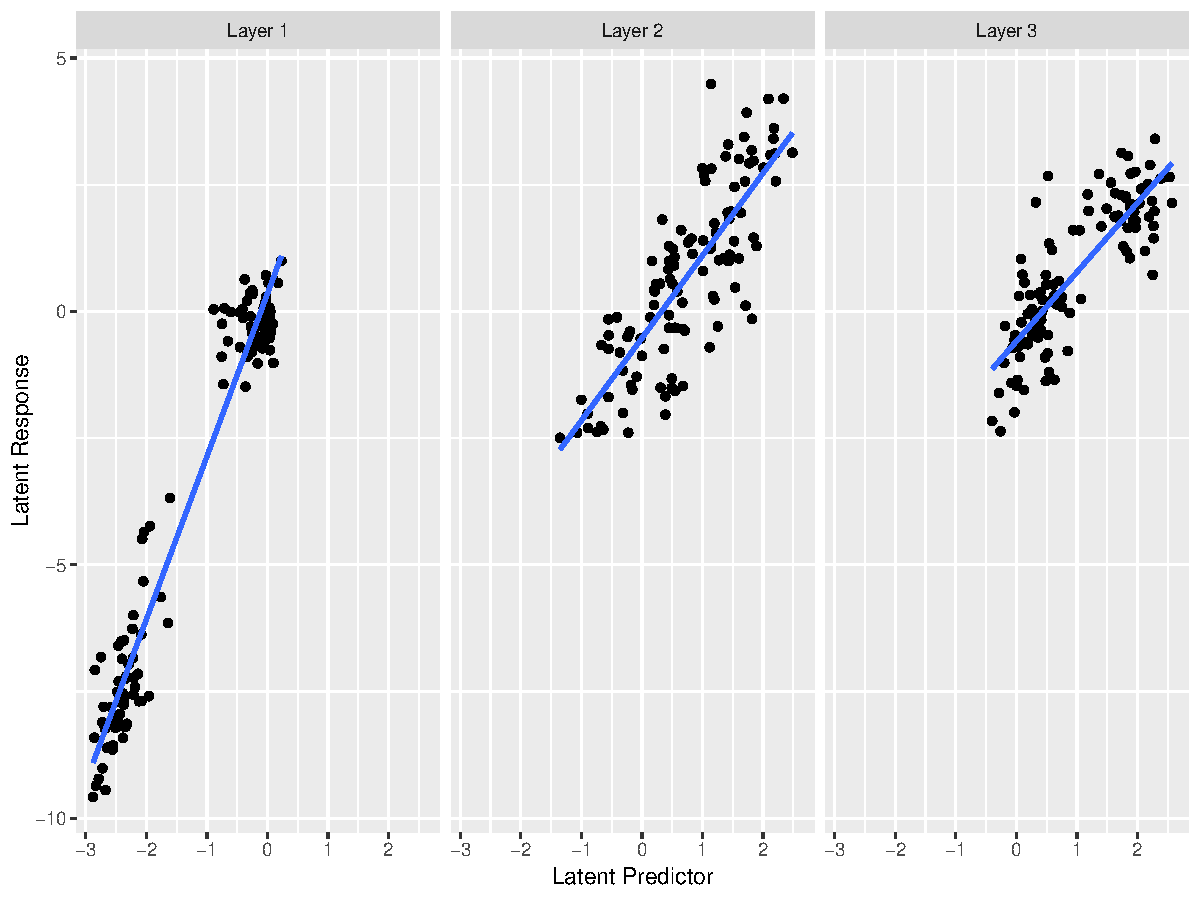
\includegraphics[width=0.75\textwidth]{./figs/letent2.pdf}
        \caption{Scatterplots of the latent responses versus the latent predictors in three SVD layers for the yeast data estimated by the SOFAR method}
    \end{figure}
\end{frame}


\begin{frame} \frametitle{Results}

    \begin{itemize}
        \item simple data analysis:
        covariance matrix of X (yes)
        the correlation between X and Y (yes)

        \item variable selection with FDR control (yes)
        
        \item FDR control (No time)
        
        \item results of regression: (Add more information)
    \end{itemize}
\end{frame}

\begin{frame}
    \frametitle{Results cont.}

    \begin{itemize}
        \item Biological interpretation and significance of our results:
        \item our results suggest:
        certain linear combination of eQTLs have effect on a subset of genes, and the groups are orthogonal. 
        may offer new information about structure of the genetic variants and gene expressions

        \item our results indicate:
        there may be 3 or 4 types of pattern in MAPK signal pathways
    \end{itemize}

\end{frame}